\FloatBarrier\newpage
\chapter{Практическая реализация}\label{ch2}


В данной главе будет рассмотрен процесс реализации системы. На основе ранее спроектированной архитектуры и выбранных инструментов будет выполнена разработка компонентов системы: мобильное приложение, backend-сервер и LLM-сервис. Исходный код разработанных компонентов системы приведены в приложениях: LLM-сервис в приложении А, backend-сервер в приложении Б и iOS-приложение в приложении В.


\section{Реализация Backend-сервера}


Backend-сервер реализован на Java с использованием Spring Boot. Он выполняет роль центрального компонента системы и отвечает за обработку запросов от iOS-приложения, реализацию бизнес-логики, взаимодействие с базой данных PostgreSQL, а также за проксирование запросов к LLM-service.


Для описания внутренней структуры backend-сервера была построена uml диаграмма классов (см. рисунок~\ref{fig:25}), где показаны основные компоненты и связи между ними. На диаграмме представлены контроллеры, сервисы, интерфейсы, репозитории, модели предметной области, DTO-объекты и компоненты безопасности.


Диаграмма отражает не только состав основных классов, но и используемые архитектурные принципы. В частности, контроллеры взаимодействуют не с конкретными реализациями сервисов, а с их интерфейсами, что соответствует принципу инверсии зависимостей и упрощает тестирование и сопровождение системы.


\begin{figure}[H]
	\centering
	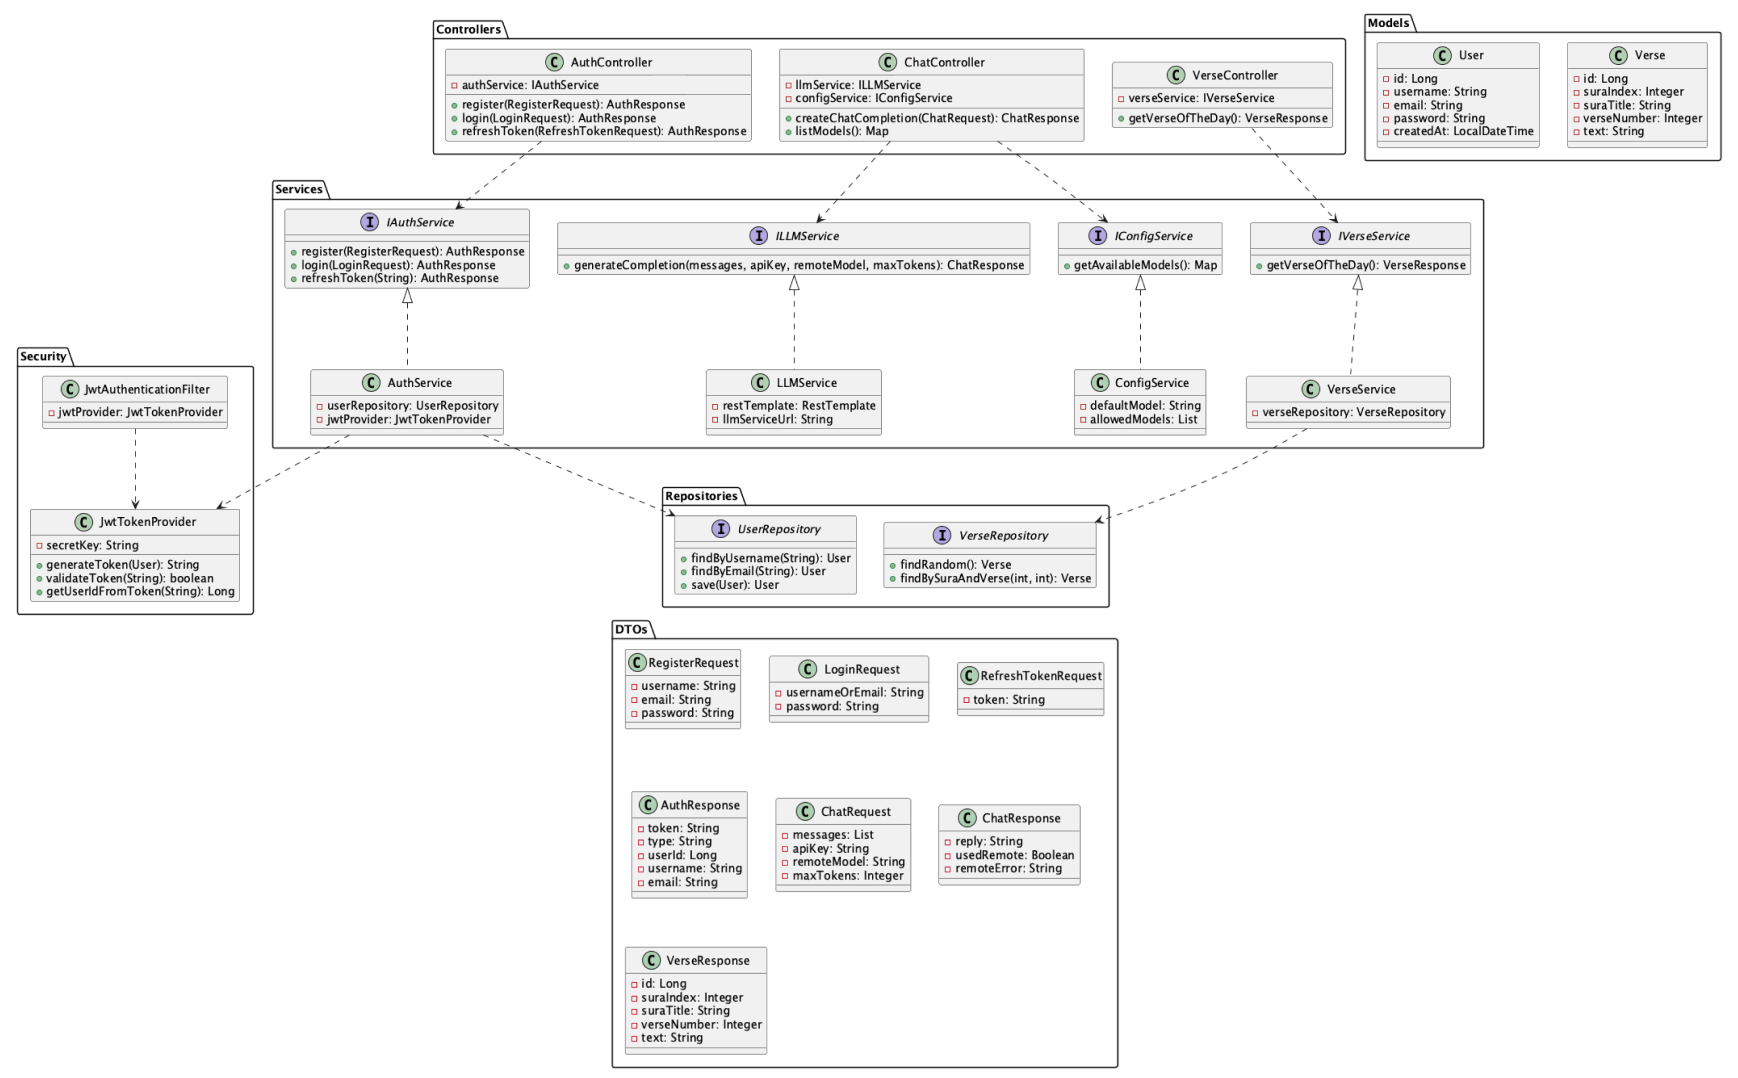
\includegraphics[width=0.85\linewidth]{my_folder/images/image25}
	\caption{Диаграмма классов backend-сервера}
	\label{fig:25}
\end{figure}


На диаграммы видно, что backend-сервер разделен на несколько логических уровней.


На уровне контроллеров расположены классы AuthController, ChatController и VerseController. Они принимают HTTP-запросы от клиента, выполняют валидацию входных данных и передают обработку в сервисный слой. Каждый контроллер взаимодействует с системой через интерфейсы сервисов (IAuthService, ILLMService, IConfigService, IVerseService), что позволяет снизить связанность компонентов и реализовать принцип инверсии зависимостей (Dependency inversion principle).


Сервисный слой содержит основную бизнес-логику приложения. Класс AuthService реализует операции регистрации, аутентификации и обновления токена, используя репозиторий пользователей и компонент генерации JWT. Класс LLMService отвечает за взаимодействие с внешним LLM-service, включая отправку запросов на генерацию ответа. Дополнительно выделен ConfigService, который инкапсулирует конфигурацию системы, в частности список доступных моделей и значение модели по умолчанию. Это позволяет отделить конфигурационные данные от логики работы чат-сервиса. Класс VerseService реализует работу с данными Корана, включая получение случайного аята дня.


Слой доступа к данным представлен интерфейсами UserRepository и VerseRepository, которые используются сервисами для взаимодействия с базой данных PostgreSQL. Для хранения и передачи данных между слоями применяются DTO-объекты (RegisterRequest, LoginRequest, ChatRequest, AuthResponse, ChatResponse, VerseResponse), что позволяет изолировать внутреннюю модель данных от внешнего API.


Отдельно на диаграмме представлены компоненты безопасности JwtTokenProvider и JwtAuthenticationFilter. Они обеспечивают генерацию, проверку и извлечение данных из JWT-токенов, а также выполняют аутентификацию входящих запросов. Это позволяет реализовать безопасный доступ к защищенным endpoint-ам без необходимости обращения к базе данных при каждом запросе.


Таким образом, представленная диаграмма классов демонстрирует, что backend-сервер реализован в соответствии с принципами модульности, слабой связанности и разделения ответственности, что обеспечивает масштабируемость и устойчивость системы к изменениям. Полный код backend-сервера приведен в приложении Б.


\section{Реализация LLM-сервиса}


\subsection{Основные компоненты сервиса}


LLM-сервис реализован в виде микросервиса, предназначенного для обработки запросов пользователей и генерации ответов на основе текстов Корана. Сервис построен с использованием архитектуры Retrieval-Augmented Generation (RAG), которая объединяет методы информационного поиска и генерации текста. Полный код LLM-сервиса приведен в приложении А.


Общая схема обработки запроса включает следующие этапы: пользовательский запрос поступает в API слой, затем передается в RAG-модуль для поиска релевантных фрагментов текста, после чего эти данные используются языковой моделью для генерации ответа.


Архитектура сервиса включает три основных слоя - API слой, RAG слой и LLM слой.


API слой реализован с использованием фреймворка FastAPI и обеспечивает обработку HTTP-запросов от backend-сервиса.


В рамках данного слоя реализованы следующие эндпоинты:

\begin{enumerate}
	\item /llm/health - проверка доступности сервиса.
	\item /llm/chat - основной интерфейс взаимодействия с системой.
	\item /llm/info - получение информации о сервисе.
\end{enumerate}

Бизнес-логика обработки запроса, связанных с чатов реализована в классе ChatService. Данный класс выступает в роли координирующего компонента и реализует последовательность шагов, необходимых для формирования ответа пользователю. Выполняются следующие операции:

\begin{enumerate}
	\item извлечение последнего пользовательского сообщения из истории диалога.
	\item обращение к RAG-пайплайну для поиска релевантных фрагментов Корана.
	\item преобразование найденных данных в текстовый контекст, используемый при генерации.
	\item вызов LLM-клиента для получения ответа.
	\item обработку возможных ошибок при взаимодействии с внешними сервисами.
\end{enumerate}

Также для управления зависимостями используется DependencyContainer, который реализует подход dependency injection. В контейнере хранится: экземпляр RAG-пайплайна (интерфейс IRAGPipeline), клиент для взаимодействия с языковой моделью (интерфейс ILLMClient), а также экземпляр ChatService (интерфейс IСhatService). Структура API-слоя показана на рисунке~\ref{fig:26}.


\begin{figure}[H]
	\centering
	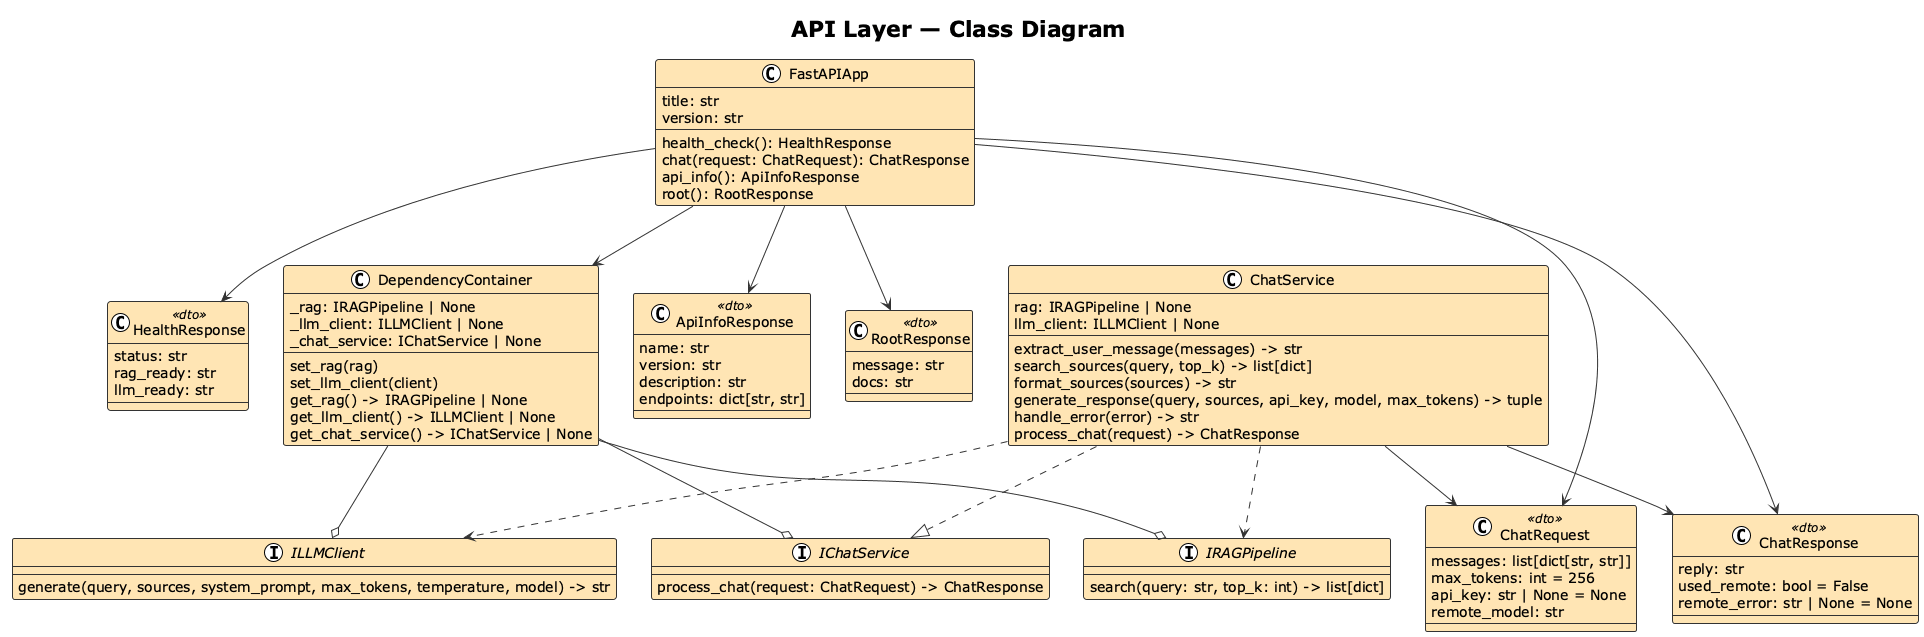
\includegraphics[width=0.85\linewidth]{my_folder/images/image26}
	\caption{Диаграмма классов api-layer у llm-сервиса}
	\label{fig:26}
\end{figure}


RAG слой отвечает за поиск релевантной информации в базе знаний и включает следующие компоненты:

\begin{enumerate}
	\item EmbeddingModel - преобразует текст в векторное представление.
	\item VectorStore -  хранит эмбеддинги документов и выполняет поиск.
	\item SimpleRAG - координирует процесс поиска.
\end{enumerate}

Обработка запроса в рамках данного слоя включает:

\begin{enumerate}
	\item Преобразование пользовательского запроса в вектор (эмбеддинг).
	\item Поиск наиболее похожих документов с использованием косинусного сходства.
	\item Выбор top-k наиболее релевантных фрагментов текста.
\end{enumerate}

Для генерации эмбеддингов используется библиотека SentenceTransformers, позволяющая учитывать семантическое сходство между текстами. Векторное хранилище реализовано в оперативной памяти, что обеспечивает высокую скорость поиска при большом объеме данных. Диаграмма классов RAG-слоя представлена на рисунке~\ref{fig:27}.


\begin{figure}[H]
	\centering
	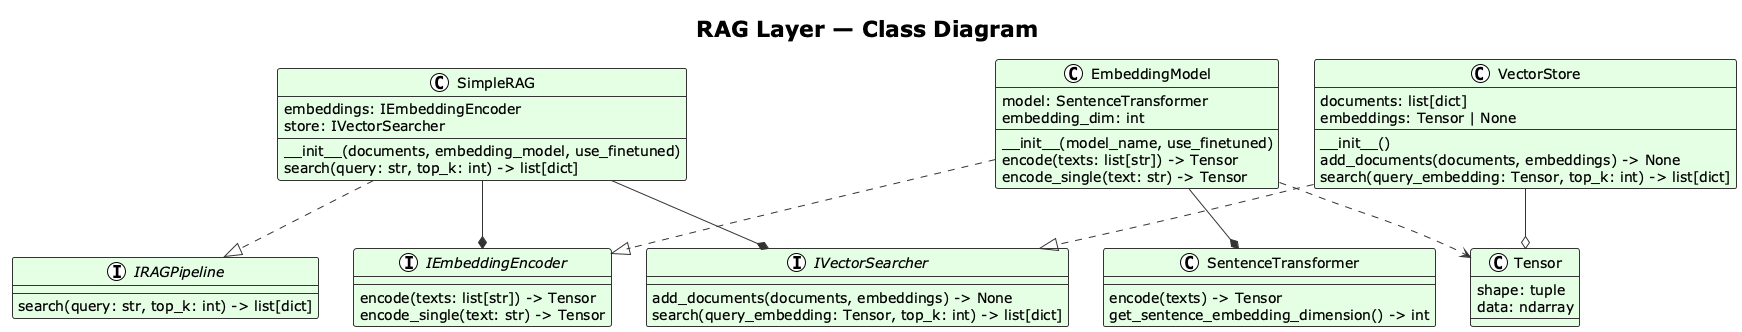
\includegraphics[width=0.85\linewidth]{my_folder/images/image27}
	\caption{Диаграмма классов rag-layer у llm-сервиса}
	\label{fig:27}
\end{figure}


LLM слой отвечает за генерацию текстового ответа на основе пользовательского запроса и найденных фрагментов. Взаимодействие с языковой моделью осуществляется через сервис OpenRouter, который предоставляет унифицированный доступ к различным моделям.


Процесс генерации включает: формирование системного промпта, добавление найденных фрагментов Корана, пользовательского запроса и отправку запроса в языковую модель вместе с получением ответа от нее (рисунок~\ref{fig:28}).


\begin{figure}[H]
	\centering
	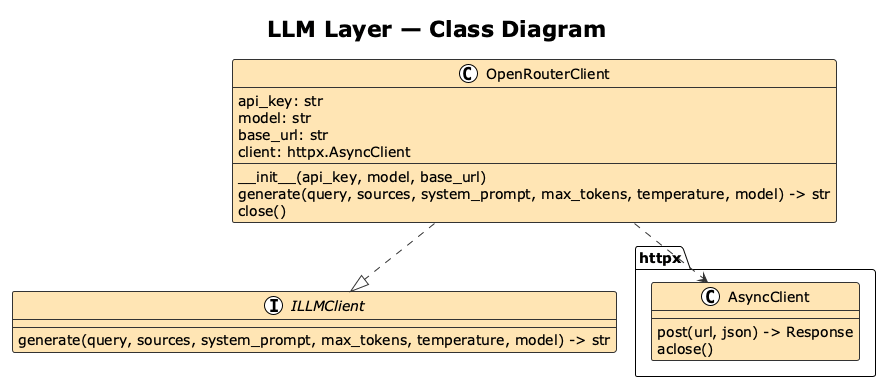
\includegraphics[width=0.85\linewidth]{my_folder/images/image28}
	\caption{Диаграмма классов rag-layer у  llm-сервиса}
	\label{fig:28}
\end{figure}


Для выполнения HTTP-запросов OpenRouterClient использует  AsyncClient. Это позволяет не блокировать взаимодействие с внешним API и эффективно обрабатывать запросов в условиях одновременной работы нескольких пользователей.


\subsection{Экспериментальный подбор параметров и моделей}


После реализации функционала в LLM-сервиса была проведена серия экспериментов, направленных на повышение качества ответов системы. Основной задачей являлась проверка сформулированных ранее гипотез, а также выбор оптимальных параметров для максимально релевантного ответа для пользователя.


Эксперименты проводились на наборе тестовых запросов, включающих вопросы, связанные с исламской культурой и Кораном:

\begin{enumerate}
	\item Что Коран говорит о запрете свинины?
	\item Какие аяты в Коране говорят о запрете алкоголя?
	\item Почему в исламе запрещен алкоголь?
	\item Что говорится в Коране о молитве и ее значении?
	\item Как в Коране описывается поведение и скромность женщины?
\end{enumerate}

Для проверки влияния ключевых параметров RAG-подсистемы был сформирован набор экспериментальных конфигураций, различающихся по двум факторам: использование retrieval-механизма и тип модели эмбеддингов.


В качестве базового сценария рассматривалась генерация ответа без использования RAG. Для сценариев с RAG дополнительно варьировались тип embedding model (базовая и fine-tuned). Конфигурации тестирования приведены в таблице~\ref{tab:rag-configs}.


\begin{table}[H]
	\centering
	\caption{Конфигурации RAG}
	\label{tab:rag-configs}
	\small
	\begin{tabular}{|p{1.0cm}|p{1.2cm}|p{9.5cm}|p{2.73cm}|}
	\hline
		No. & RAG & Embedding model & Состояние \\
	\hline
		C1 & Нет & - & - \\
	\hline
		C2 & Да & paraphrase-multilingual-mpnet-base-v2 & Base \\
	\hline
		C3 & Да & paraphrase-multilingual-mpnet-base-v2 & Fine-tuned \\
	\hline
		C4 & Да & ai-forever/sbert\_large\_nlu\_ru & Base \\
	\hline
		C5 & Да & ai-forever/sbert\_large\_nlu\_ru & Fine-tuned \\
	\hline
	\end{tabular}
\end{table}

Для оценки итогового качества ответа языковой модели использовались следующие критерии: корректность (A), обоснованность (G), полнота (C) и галлюцинации (H) (таблица~\ref{tab:answer-metrics}).

\begin{table}[H]
	\centering
	\caption{Метрики оценки ответов}
	\label{tab:answer-metrics}
	\small
	\begin{tabular}{|p{4cm}|p{4cm}|p{4cm}|}
	\hline
		Критерий & Описание & Диапазон \\
	\hline
		Корректность (A) & Насколько ответ соответствует содержанию Корана & 0 - 5 \\
	\hline
		Обоснованность (G) & Насколько ответ опирается на релевантные источники & 0 - 5 \\
	\hline
		Полнота (C) & Насколько полно раскрыт вопрос & 0 - 5 \\
	\hline
		Галлюцинации (H) & Наличие недостоверной информации & 0 - 5 \\
	\hline
	\end{tabular}
\end{table}

По каждому критерию оценка проводится по шкале от 0 до 5. Для всех критериев, кроме галлюцинаций, оценка 0 - это полное несоответствие, а 5 - идеальное соответствие. Для критерия галлюцинаций 0 - это их полное отсутствие, а 5 - большое количество недостоверной информации. Итоговая оценка качества ответа языковой модели рассчитывается по формуле:

\begin{equation}
	AnswerScore = 0{,}2 \cdot A + 0{,}3 \cdot G + 0{,}2 \cdot C - 0{,}5 \cdot H + 1
	\label{eq:answer-score}
\end{equation}

Следует отметить, что указанные критерии применялись исключительно для оценки итогового ответа языковой модели и не использовались для непосредственной оценки качества retrieval-подсистемы. Это обусловлено тем, что значение косинусного сходства, получаемое на этапе retrieval, не всегда отражает фактическую релевантность найденных аятов. В ряде случаев документы с высоким значением сходства оказывались семантически близкими к вопросу, но не содержали прямого ответа на него. В связи с этим качество retrieval оценивалось отдельно, на основе ручного анализа найденных аятов.

Для оценки качества retrieval использовались следующие критерии: релевантность найденных источников (R) и точность top-3 выдачи (T) (таблица~\ref{tab:retrieval-metrics}).

\begin{table}[H]
	\centering
	\caption{Метрики оценки поиска}
	\label{tab:retrieval-metrics}
	\small
	\begin{tabular}{|p{4cm}|p{4cm}|p{4cm}|}
	\hline
		Критерий & Описание & Диапазон \\
	\hline
		Релевантность источников (R) & Насколько найденные аяты действительно соответствуют поставленному вопросу & 0 - 5 \\
	\hline
		Точность top-3 выдачи (T) & Доля релевантных аятов среди первых трех найденных документов по всем заданным вопросам & 0 - 5 \\
	\hline
	\end{tabular}
\end{table}

Оценка retrieval проводится вручную. Для каждого вопроса анализируются первые три аята, возвращённые retrieval-подсистемой. При оценке учитывается, содержат ли найденные аяты прямой ответ на поставленный вопрос, являются ли они частично релевантными либо не относятся к запрашиваемой теме вообще.

Показатель точности top-3 выдачи рассчитывается по формуле:

\begin{equation}
	t_i = \frac{N_{rel}}{3} \times 5
	\label{eq:top3-single}
\end{equation}

где $N_{rel}$ - это количество релевантных аятов среди первых трех найденных документов.

Оценка всех вопросов считается по формуле:

\begin{equation}
	T = \frac{1}{5} \times \sum_{i=1}^{5} t_i
	\label{eq:top3-avg}
\end{equation}

Итоговая оценка качества retrieval определяется по формуле:

\begin{equation}
	RetrievalScore = 0.6R + 0.4T
	\label{eq:retrieval-score}
\end{equation}

Общая оценка экспериментальной конфигурации рассчитывалась с учетом как качества retrieval, так и качества итогового ответа языковой модели:

\begin{equation}
	FinalScore = 0.4 \times RetrievalScore + 0.6 \times AnswerScore
	\label{eq:final-score}
\end{equation}

Таким образом, оценка каждой экспериментальной конфигурации выполнялась в два этапа. На первом этапе анализировалось качество retrieval-подсистемы по найденным аятам, на втором - качество итогового ответа языковой модели.

\begin{table}[H]
	\centering
	\caption{Результаты тестирования конфигураций RAG}
	\label{tab:rag-results}
	\small
	\resizebox{\textwidth}{!}{
\begin{tabular}{|p{2.5cm}|c|c|p{2cm}|c|c|c|c|p{2cm}|p{2cm}|}
	\hline
		Конфигурация & R & T & Retrieval Score & A & G & C & H & Answer Score & Final Score \\
	\hline
		C1 & 0 & 0 & 0 & 4 & 3 & 3 & 1 & 2,8 & 2,8 \\
	\hline
		C2 & 3 & 3 & 3 & 4 & 3 & 5 & 1 & 3,2 & 3,12 \\
	\hline
		C3 & 3 & 4 & 3,4 & 5 & 4 & 4 & 0 & 4 & 3,76 \\
	\hline
		C4 & 1 & 1 & 1 & 4 & 3 & 4 & 1 & 3 & 2,2 \\
	\hline
		C5 & 3 & 3 & 3 & 4 & 4 & 5 & 1 & 3,5 & 3,3 \\
	\hline
	\end{tabular}
}
\end{table}


Результаты проведенных экспериментов, представленные в таблице~\ref{tab:rag-results}, позволяют сделать выводы о влиянии рассматриваемых факторов на качество работы системы.


Прежде всего, сравнение базовой конфигурации C1 с конфигурациями, использующими retrieval-механизм (C2--C5), показывает, что применение RAG-подсистемы в целом положительно влияет на качество ответов. Несмотря на то, что языковая модель в конфигурации C1 демонстрирует приемлемые значения корректности и полноты, отсутствие опоры на конкретные источники приводит к снижению обоснованности ответов и увеличению риска появления галлюцинаций. В конфигурациях с использованием RAG наблюдается рост показателя обоснованности, что связано с использованием релевантных аятов при генерации ответа.


Анализ качества retrieval-подсистемы показывает, что эффективность поиска существенно зависит от используемой embedding модели. Конфигурации C2 и C4, использующие базовые версии моделей, демонстрируют более низкие значения показателей R и T по сравнению с соответствующими дообученными. Это говорит о том, что базовые модели не всегда способны корректно учитывать семантические особенности религиозных текстов, что приводит к включению нерелевантных аятов в выдачу. В то же время конфигурации C3 и C5, использующие дообученные модели эмбеддингов, показывают более высокие значения показателей релевантности и точности top-3 выдачи. Это подтверждает, что дообучение модели на специализированном корпусе позволяет существенно повысить качество семантического поиска и уменьшить количество нерелевантных документов.


Также сравнение архитектур embedding моделей показывает, что модель paraphrase-multilingual-mpnet-base-v2 демонстрирует более высокие результаты по сравнению с ai-forever/sbert\_large\_nlu\_ru как в базовом, так и в дообученном состоянии. Особенно заметно это проявляется в конфигурации C3, которая достигает наибольшего значения итоговой оценки среди всех рассмотренных вариантов.


Полученные результаты позволяют подтвердить сформулированные гипотезы. Вместе с тем проведенное экспериментальное исследование имеет ряд ограничений. Набор тестовых запросов ограничен и не охватывает все возможные сценарии использования системы. В дальнейшем планируется расширение корпуса тестовых данных, а также автоматизация оценки качества.


Гипотеза 1 о том, что применение RAG повышает качество ответов и снижает частоту галлюцинаций подтверждается. Конфигурации с использованием RAG демонстрируют более высокие значения показателя обоснованности за счет опоры на релевантные источники. Однако полностью устранить галлюцинации не удается, модель продолжает генерировать частично некорректные формулировки, включая искажения религиозной терминологии.


Гипотеза 2 о влиянии дообучения embedding модели также подтверждается. Во всех случаях дообученные модели (C3 и C5) демонстрируют более высокое качество retrieval и, следовательно, более высокие итоговые оценки по сравнению с соответствующими базовыми моделями (C2 и C4).


На основании проведенного исследования для дальнейшей разработки была выбрана конфигурация, показавшая наилучшие результаты, а именно модель paraphrase-multilingual-mpnet-base-v2, дообученная на специализированном корпусе.


\section{Реализация iOS-приложения}


Клиентская часть системы реализована в виде iOS-приложения. В процессе разработки были реализованы функциональные модули аутентификации, домашнего экрана, чата с AI-ассистентом, сканирования ингредиентов, чтения Корана, расчета времени молитвы и настроек приложения. Структурно проект разделен на модули App, Navigation, Features, Core, Resources и Models, что позволяет разграничить пользовательский интерфейс, навигацию, бизнес-логику и инфраструктурные компоненты. Полный код iOS-приложения приведен в приложении В.


\subsection{Структура проекта}


Основная прикладная логика сосредоточена в Features, где каждая функциональная область оформлена как отдельный модуль. Так, модуль Auth отвечает за сценарии входа и регистрации, Home реализует главный экран приложения, Chat содержит экран взаимодействия с AI-ассистентом, Scanner предназначен для анализа состава продуктов, Quran обеспечивает просмотр сур и аятов, а Prayer реализует расчет времени молитвы и настройку уведомлений. Отдельно выделен модуль Settings, предназначенный для управления пользовательскими параметрами приложения (рисунок~\ref{fig:29}).


\begin{figure}[H]
	\centering
	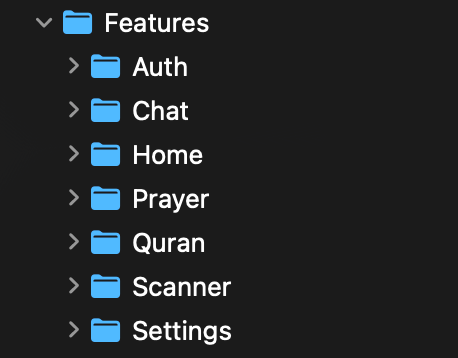
\includegraphics[width=0.85\linewidth]{my_folder/images/image29}
	\caption{Модуль Features}
	\label{fig:29}
\end{figure}


Общая навигация приложения реализована в модуле Navigation, включающем главный координатор, корневой RouterView и координаторы для отдельных разделов приложения (рисунок~\ref{fig:31}). Общие компоненты вынесены в модуль Core, где реализованы сетевой слой, сервис геолокации, переиспользуемые UI-компоненты и вспомогательные расширения (рисунок~\ref{fig:30}).


\begin{figure}[H]
	\centering
	
\includegraphics[width=0.85\linewidth]{my_folder/images/image30}
	\caption{Модуль Core}
	\label{fig:30}
\end{figure}


\begin{figure}[H]
	\centering
	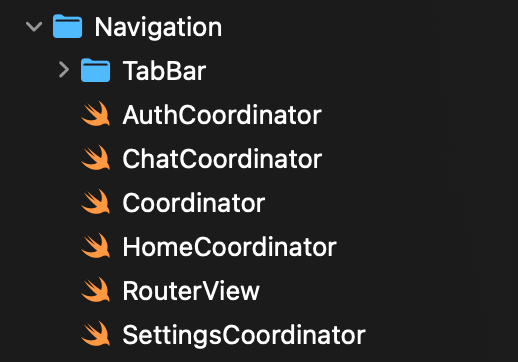
\includegraphics[width=0.85\linewidth]{my_folder/images/image31}
	\caption{Модуль Navigation}
	\label{fig:31}
\end{figure}


\subsection{Реализация навигации}


Навигация в приложении реализована в модуле Navigation. В состав данного модуля входят главный класс Coordinator, корневое представление RouterView, а также координаторы HomeCoordinator, ChatCoordinator, SettingsCoordinator и AuthCoordinator. Дополнительно в навигационный слой включены компоненты TabBarItem и TabBarView, отвечающие за организацию переключения между основными разделами приложения.


Coordinator управляет стеком переходов и текущей выбранной вкладкой приложения. За счет этого навигация становится централизованной: экраны не создают и не открывают другие экраны напрямую, а только инициируют переход через методы координатора. Корневой контейнер навигации реализован в RouterView. Он связывает состояние координатора с интерфейсом приложения и обеспечивает отображение соответствующего стека экранов. Через RouterView пользователь может переключаться между основными вкладками приложения, а также переходить к вложенным экранам внутри отдельных функциональных модулей.


Для маршрутизации внутри отдельных разделов приложения используются специализированные координаторы. HomeCoordinator отвечает за переходы, связанные с главным экраном, сканером, списком сур, чтением суры и настройками молитвы. ChatCoordinator управляет экраном диалога с AI-ассистентом. SettingsCoordinator содержит маршруты, относящиеся к настройкам приложения. AuthCoordinator используется для сценариев авторизации, включая вход и регистрацию пользователя.


Отдельно реализован механизм переключения между основными вкладками приложения. Для этого используются TabBarItem, задающий набор доступных вкладок, и TabBarView, отвечающий за отображение панели навигации. В текущей реализации выделены три основные вкладки: Главный экран(Home), Чат(Chat) и Настройки(Settings) (рисунок~\ref{fig:32}).


\begin{figure}[H]
	\centering
	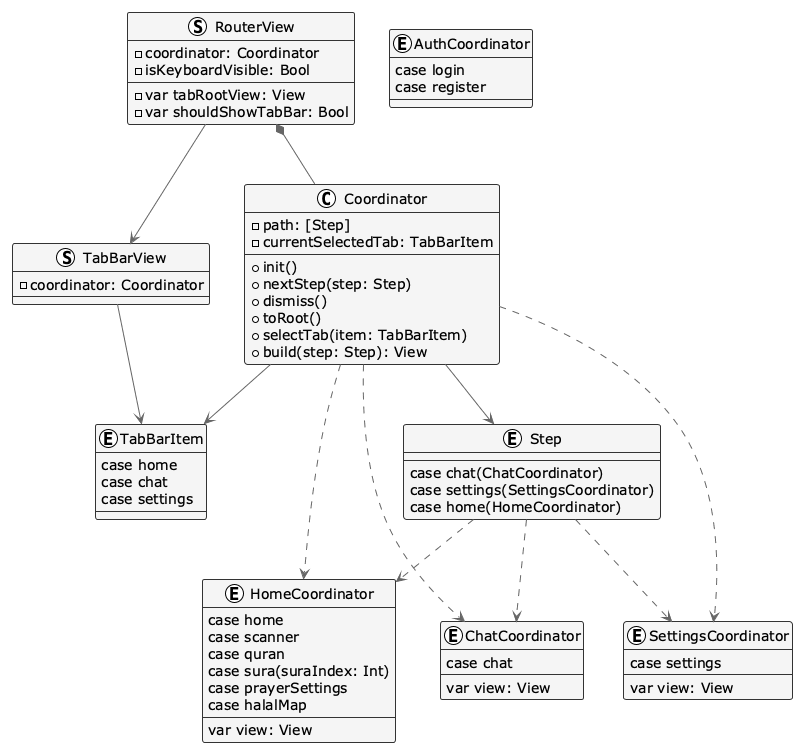
\includegraphics[width=0.85\linewidth]{my_folder/images/image32}
	\caption{UML-диаграмма классов модуля навигации}
	\label{fig:32}
\end{figure}


\subsection{Реализация функциональных модулей.}


Каждый модуль оформлен как отдельная часть проекта и включает собственные представления, модели и сервисы. Это позволяет изолировать различные области функциональности друг от друга и упрощает дальнейшее масштабирование приложения. В текущей реализации выделены модули Auth, Home, Chat, Scanner, Quran, Prayer и Settings.


Создание экранов в приложении реализовано централизованно через ScreenFactoryImpl, который выступает фабрикой пользовательских представлений. Для каждого основного сценария в нем предусмотрен отдельный метод, возвращающий уже сконфигурированный экран, например makeLoginView(), makeChatView(), makeScannerView(), makeHomeView() и другие. Внутри фабрики используется DependencyContainer, который инициализирует основные сервисы приложения и предоставляет их экранным модулям. За счет этого зависимости передаются в представления через конструктор, а не создаются непосредственно внутри экранов.


\subsubsection{Модуль аутентификации}


Модуль аутентификации отвечает за вход и регистрацию пользователя. В нем содержатся модели данных, сервис взаимодействия с backend и пользовательские экраны авторизации. Данный модуль обеспечивает переход между гостевым режимом и полным режимом работы приложения, в котором пользователю становятся доступны персонализированные функции системы. Управление состоянием авторизации выполняется через AuthManager, а сетевое взаимодействие через AuthService (рисунки~\ref{fig:33},~\ref{fig:34}).


\begin{figure}[H]
	\centering
	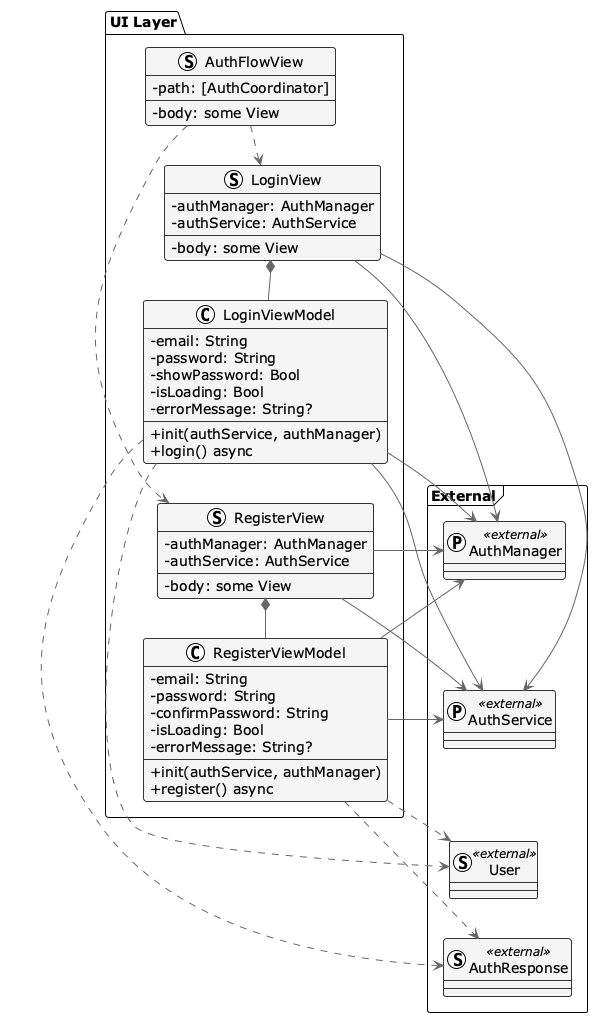
\includegraphics[width=0.85\linewidth]{my_folder/images/image33}
	\caption{UML-диаграмма классов модуля аутентификации. UI}
	\label{fig:33}
\end{figure}


\begin{figure}[H]
	\centering
	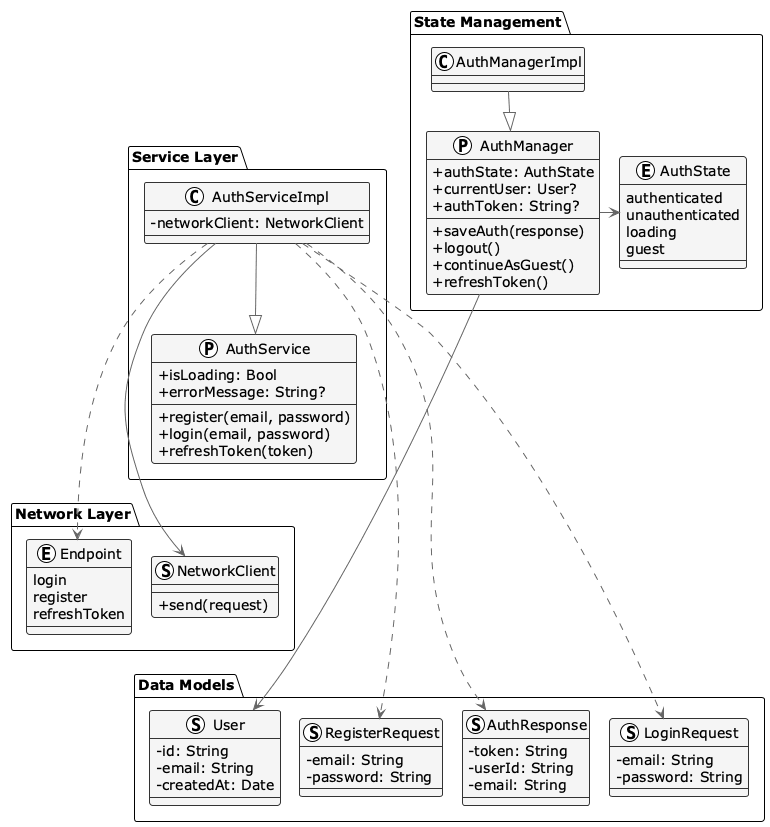
\includegraphics[width=0.85\linewidth]{my_folder/images/image34}
	\caption{UML-диаграмма классов модуля аутентификации. Services}
	\label{fig:34}
\end{figure}


\subsubsection{Модуль главного экрана}


Модуль Home реализует главный экран приложения и служит основной точкой входа в остальные пользовательские сценарии. На главном экране отображаются ключевые элементы интерфейса: карточка со случайным аятом, карточка времени молитвы, баннер гостевого режима и кнопки быстрого перехода к основным функциям приложения.


\subsubsection{Модуль чата}


Модуль Chat является одной из ключевых частей приложения, он реализует взаимодействие пользователя с AI-ассистентом. Данный модуль включает экран диалога, модели сообщений, визуальные компоненты отображения переписки и сервис отправки запросов на backend. Пользователь может вводить сообщения в свободной форме, после чего текст запроса передается на серверную часть.


На уровне взаимодействия с системой чат опирается на backend API. Клиент не обращается напрямую к LLM-service, а отправляет запросы на основной backend, который уже проксирует их в соответствующий сервис. Это позволяет скрыть от клиента внутреннюю организацию серверной части и сохранить единый интерфейс взаимодействия для мобильного приложения. Кроме того, в модуле предусмотрена поддержка выбора модели, что связано с использованием OpenRouter в серверной части системы (рисунок~\ref{fig:35}).


\begin{figure}[H]
	\centering
	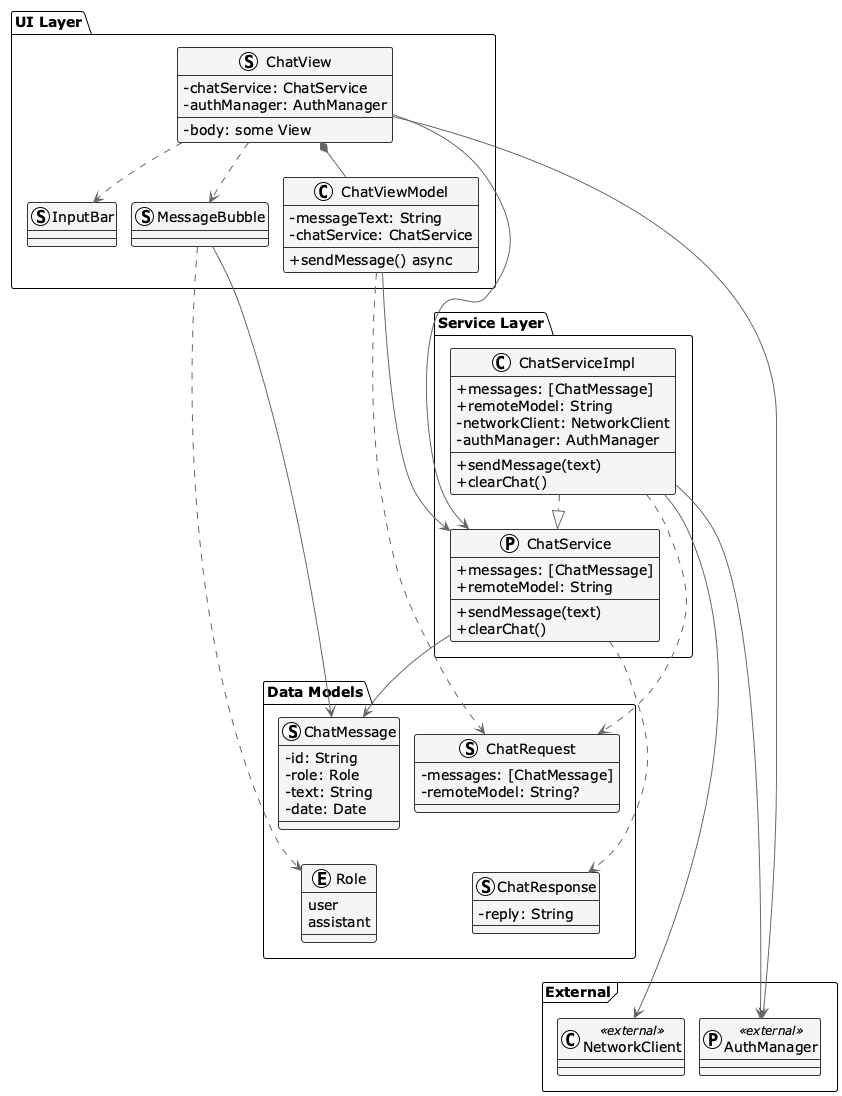
\includegraphics[width=0.85\linewidth]{my_folder/images/image35}
	\caption{UML-диаграмма классов модуля чата}
	\label{fig:35}
\end{figure}


\subsubsection{Модуль сканирования ингредиентов}


Модуль Scanner предназначен для анализа состава продуктов и и выявления в них запрещенных в исламе ингредиентов.


Структура модуль включает экран ScannerView, модель представления ScannerViewModel и сервис IngredientService. Экран отвечает за взаимодействие с пользователем и предоставляет несколько вариантов ввода данных: получение изображения через камеру, выбор фотографии из галереи и ручной ввод текста состава. ScannerViewModel управляет состоянием экрана, координирует распознавание текста и инициирует анализ. IngredientService отвечает за загрузку базы ингредиентов и сопоставление распознанного текста с данными этой базы.


На первом этапе пользователь передает состав продукта одним из доступных способов. Если используется изображение, далее запускается OCR-распознавание текста средствами Vision Framework. Распознанный текст передается в сервис анализа, который извлекает названия ингредиентов и выполняет их сопоставление с внутренней базой ингредиентов. По результатам сопоставления формируется объект ProductAnalysis, содержащий перечень найденных ингредиентов, их статусы и общий итоговый результат для продукта.


При анализе учитываются как текстовые названия ингредиентов, так и пищевые добавки, обозначенные E-кодами. Для каждого обнаруженного элемента определяется его статус, после чего вычисляется итоговый статус всего продукта. Если среди найденных компонентов присутствует хотя бы один харам-ингредиент, общий результат помечается как "харам". Если запрещенных компонентов нет, но присутствуют сомнительные, продукт получает статус "сомнительный". В случае, когда все распознанные ингредиенты относятся к разрешенным, результат помечается как "халяль". Такой подход соответствует логике, ранее заложенной в алгоритме анализа состава продукта (рисунок~\ref{fig:36}).


\begin{figure}[H]
	\centering
	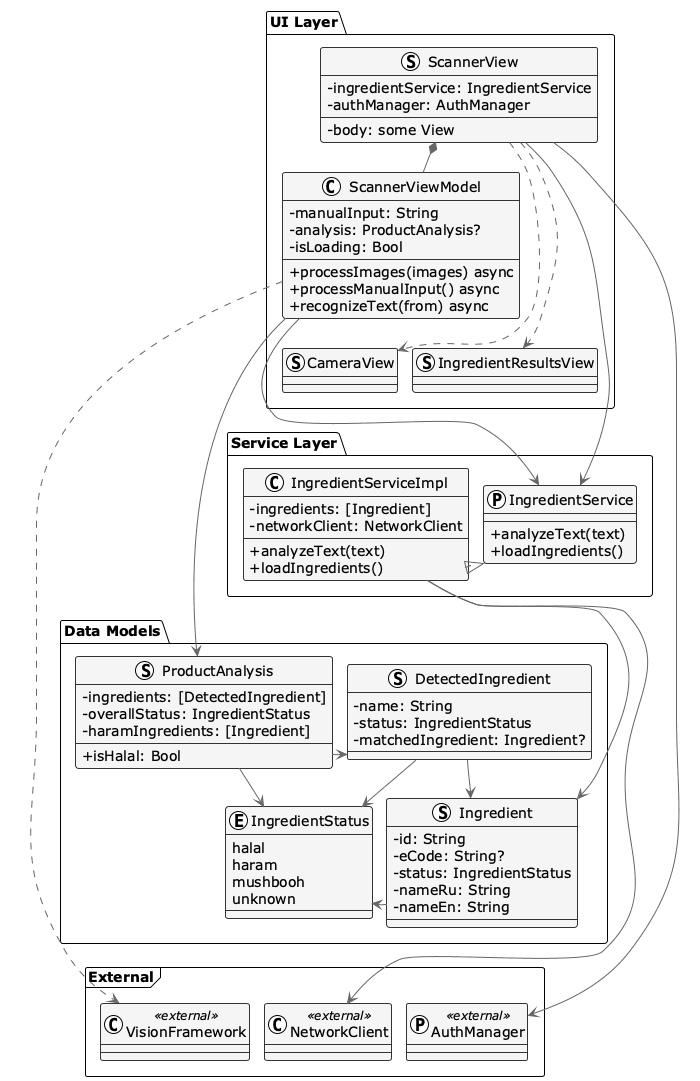
\includegraphics[width=0.85\linewidth]{my_folder/images/image36}
	\caption{UML-диаграмма классов модуля сканирования ингредиентов}
	\label{fig:36}
\end{figure}


\subsubsection{Модуль чтения Корана}


Модуль Quran предназначен для работы с текстом Корана: просмотр списка сур и чтение выбранной суры. В состав модуля входят сервис хранения QuranStorageService, экран со списком сур QuranListView и экран чтения SuraReaderView.


Основой модуля является QuranStorageService, который отвечает за загрузку текста Корана из локальных ресурсов приложения и сохранение прогресса чтения пользователя. В текущей реализации данные загружаются из ресурсов, включенных в приложение, а информация о последней прочитанной суре и позиции чтения сохраняется локально.


Экран QuranListView предназначен для отображения полного списка сур и поиска по ним. Для управления состоянием используется QuranListViewModel.


Экран SuraReaderView реализует чтение конкретной суры. Связанная с ним SuraReaderViewModel получает нужную суру из хранилища, управляет параметрами отображения и отслеживает прогресс чтения. При необходимости текущее положение пользователя сохраняется (рисунок~\ref{fig:37}).


\begin{figure}[H]
	\centering
	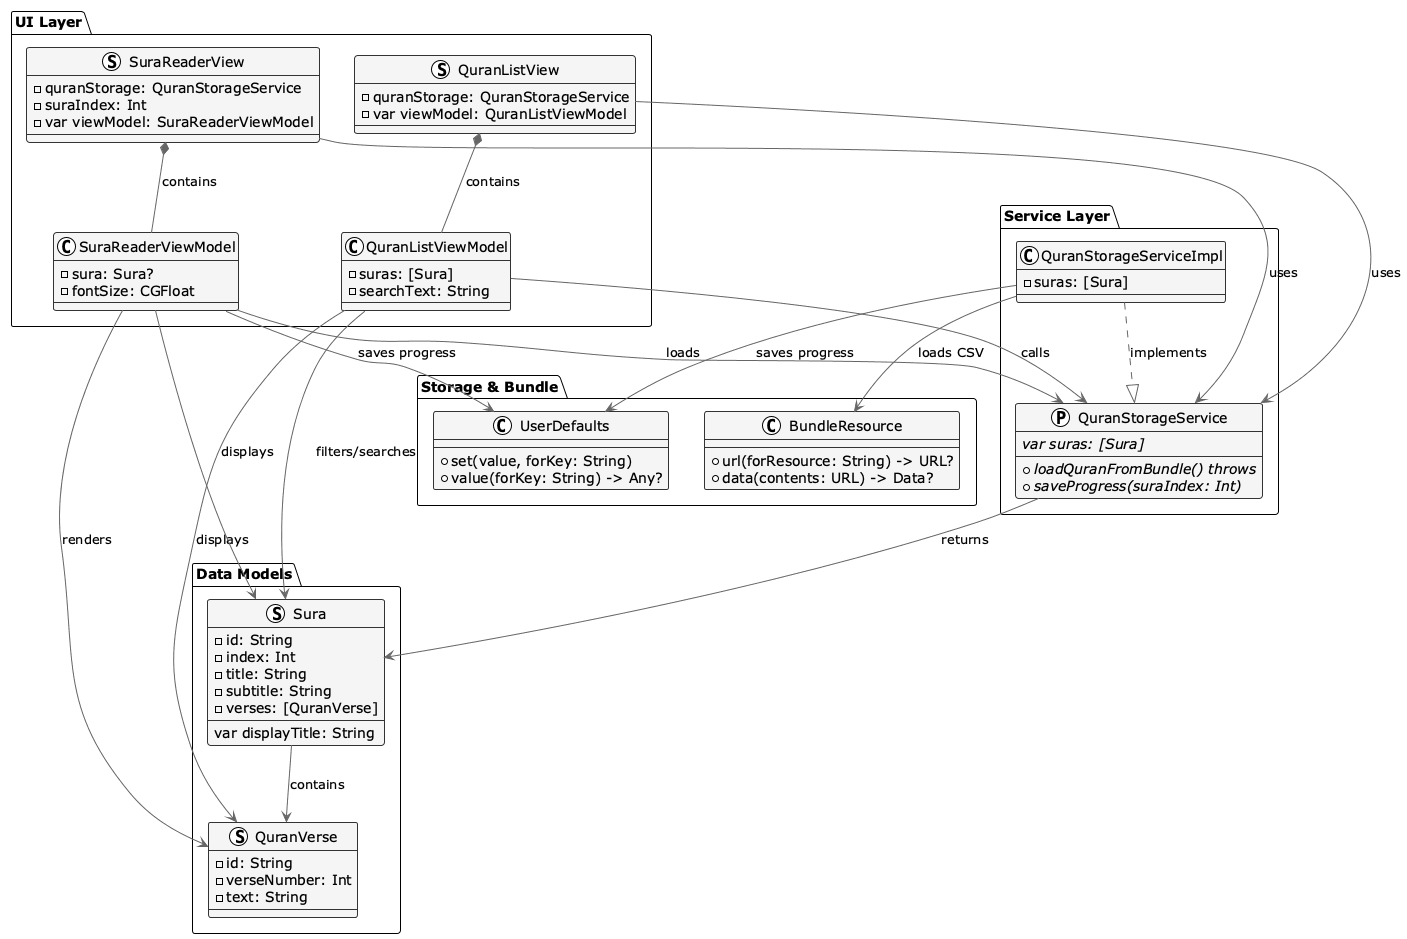
\includegraphics[width=0.85\linewidth]{my_folder/images/image37}
	\caption{UML-диаграмма классов модуля чтения Корана}
	\label{fig:37}
\end{figure}


\subsubsection{Модуль времени молитвы}


Модуль Prayer отвечает за расчет времени молитвы, отображение расписания на текущий день, определение ближайшей молитвы и настройку уведомлений. В состав модуля входят сервис расчета времени молитвы PrayerTimeService, сервис уведомлений PrayerNotificationService, сервис геолокации LocationService, хранилище настроек PrayerSettingsStore, а также пользовательские экраны PrayerTimesCardView и PrayerNotificationSettingsView.


Центральным элементом модуля является PrayerTimeService, который отвечает за вычисление расписания молитв на основе текущих координат пользователя, даты и выбранного метода расчета. В реализации для этих вычислений используется библиотека Adhan, предоставляющая готовые алгоритмы расчета времени намаза на основе астрономических параметров.


Результатом работы сервиса является структура DailyPrayerTimes, содержащая время пяти обязательных молитв: fajr, dhuhr, asr, maghrib и isha. Также на основе полученного расписания определяется ближайшая предстоящая молитва.


Для получения координат используется LocationService, представляющий собой обертку над системным фреймворком CoreLocation. После запроса разрешения у пользователя сервис получает текущее местоположение и передает его в модуль расчета времени молитвы.


Отдельная часть модуля связана с хранением пользовательских параметров. В PrayerSettingsStore сохраняются выбранный метод расчета, мазхаб (правовая школа в исламе) и настройки уведомлений.


Для напоминаний о времени молитвы используется PrayerNotificationService. Он запрашивает разрешение на отправку уведомлений, формирует локальные уведомления и позволяет пересоздавать их при изменении пользовательских настроек.


На уровне интерфейса основным элементом является PrayerTimesCardView, связанный с PrayerTimesCardViewModel. Эта модель представления получает данные из сервисов, управляет состоянием экрана и передает в интерфейс рассчитанное расписание, а также информацию о ближайшей молитве (рисунки~\ref{fig:38},~\ref{fig:39}).


\begin{figure}[H]
	\centering
	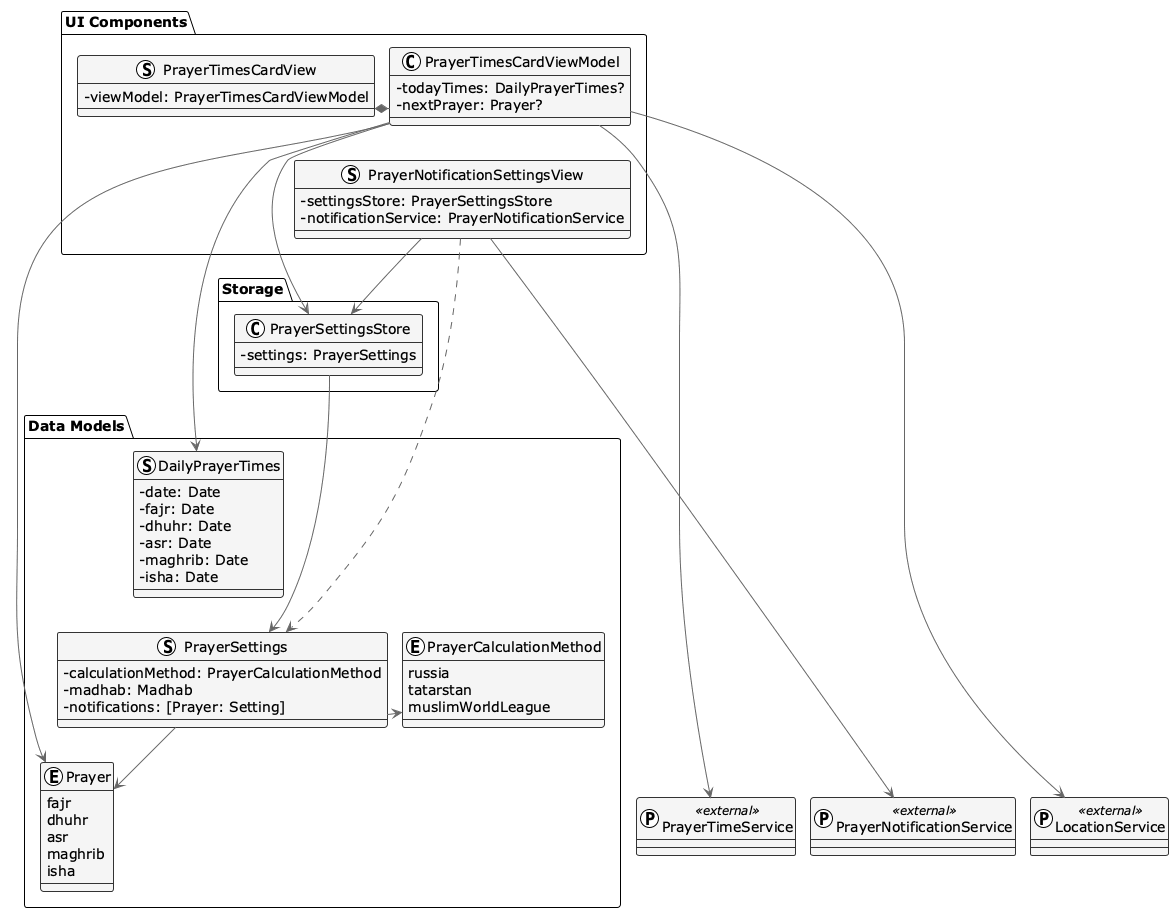
\includegraphics[width=0.85\linewidth]{my_folder/images/image38}
	\caption{UML-диаграмма классов модуля времени молитвы. UI}
	\label{fig:38}
\end{figure}


\begin{figure}[H]
	\centering
	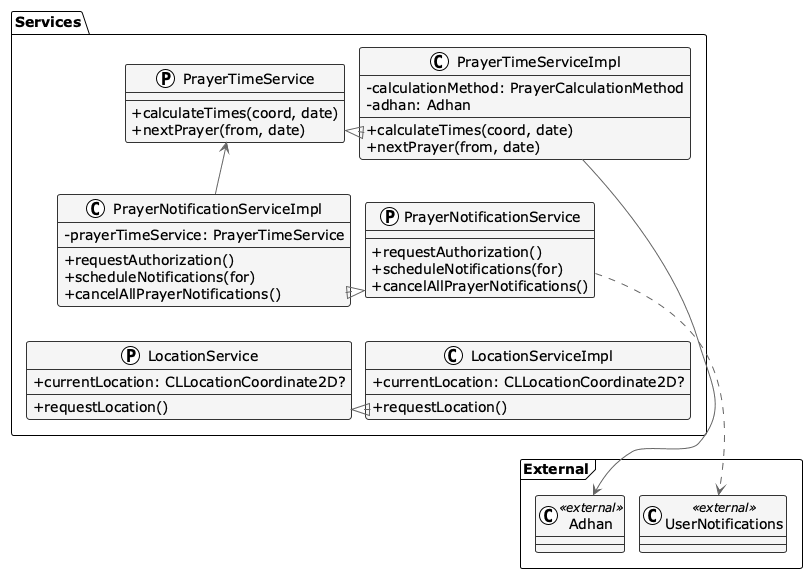
\includegraphics[width=0.85\linewidth]{my_folder/images/image39}
	\caption{UML-диаграмма классов модуля времени молитвы. Services}
	\label{fig:39}
\end{figure}


\subsubsection{Модуль настроек}


Модуль Settings предназначен для управления параметрами приложения и завершает набор основных пользовательских сценариев клиентской части. Через данный раздел пользователь получает доступ к настройкам, связанным с профилем, параметрами работы чата и управлением авторизацией. В состав модуля входят экран SettingsView, модель представления SettingsViewModel, а также вспомогательный компонент RemoteModelSettingsSection, отвечающий за настройку параметров удаленной языковой модели.


С точки зрения архитектуры модуль настроек взаимодействует прежде всего с двумя сервисами: ChatService и AuthManager. AuthManager предоставляет сведения о текущем пользователе и его статусе, а также используется для выполнения выхода из аккаунта. ChatService, в свою очередь, отвечает за параметры работы AI-ассистента, включая выбор удаленной модели, ограничение на количество токенов, температурный параметр генерации и использование режима RAG.


На уровне интерфейса SettingsView объединяет несколько групп параметров. Во-первых, здесь отображается информация о текущем пользователе, если приложение работает в авторизованном режиме. Во-вторых, пользователю предоставляется возможность изменять параметры удаленной языковой модели. Для этого используется отдельный компонент RemoteModelSettingsSection, который инкапсулирует элементы управления, связанные с выбором модели и настройками генерации. Модель представления SettingsViewModel управляет состоянием экрана и связывает элементы интерфейса с соответствующими параметрами сервисов. Через нее поддерживается изменение значений, связанных с отображением API-ключа, ограничением числа токенов, температурой генерации и выбором пользовательской модели.


\subsection{Реализация сетевого взаимодействия}


Взаимодействие iOS-приложения с серверной частью реализовано через отдельный сетевой слой, вынесенный в модуль Core/Network. Это позволяет отделить логику пользовательских модулей от деталей HTTP-коммуникации и обеспечить единый механизм работы с backend API. В состав сетевого слоя входят компоненты NetworkClient, APIConfiguration, APIRequest, Endpoint и NetworkError.


NetworkClient выполняет отправку запросов и получение ответов от backend-сервера. Его задача заключается в том, чтобы инкапсулировать общую логику формирования HTTP-запросов, обработки ответов, декодирования JSON и обработки сетевых ошибок. Благодаря этому прикладные сервисы, такие как AuthService и ChatService, не работают напрямую с URLSession, а используют унифицированный клиент.


Для описания запросов используется абстракция APIRequest, а перечисление Endpoint задает набор доступных маршрутов backend-сервера.


Все сетевые операции в приложении реализованы с использованием URLSession и механизма async/await. Это позволяет выполнять запросы асинхронно, не блокируя основной поток и не нарушая отзывчивость пользовательского интерфейса (рисунок~\ref{fig:40}).


\begin{figure}[H]
	\centering
	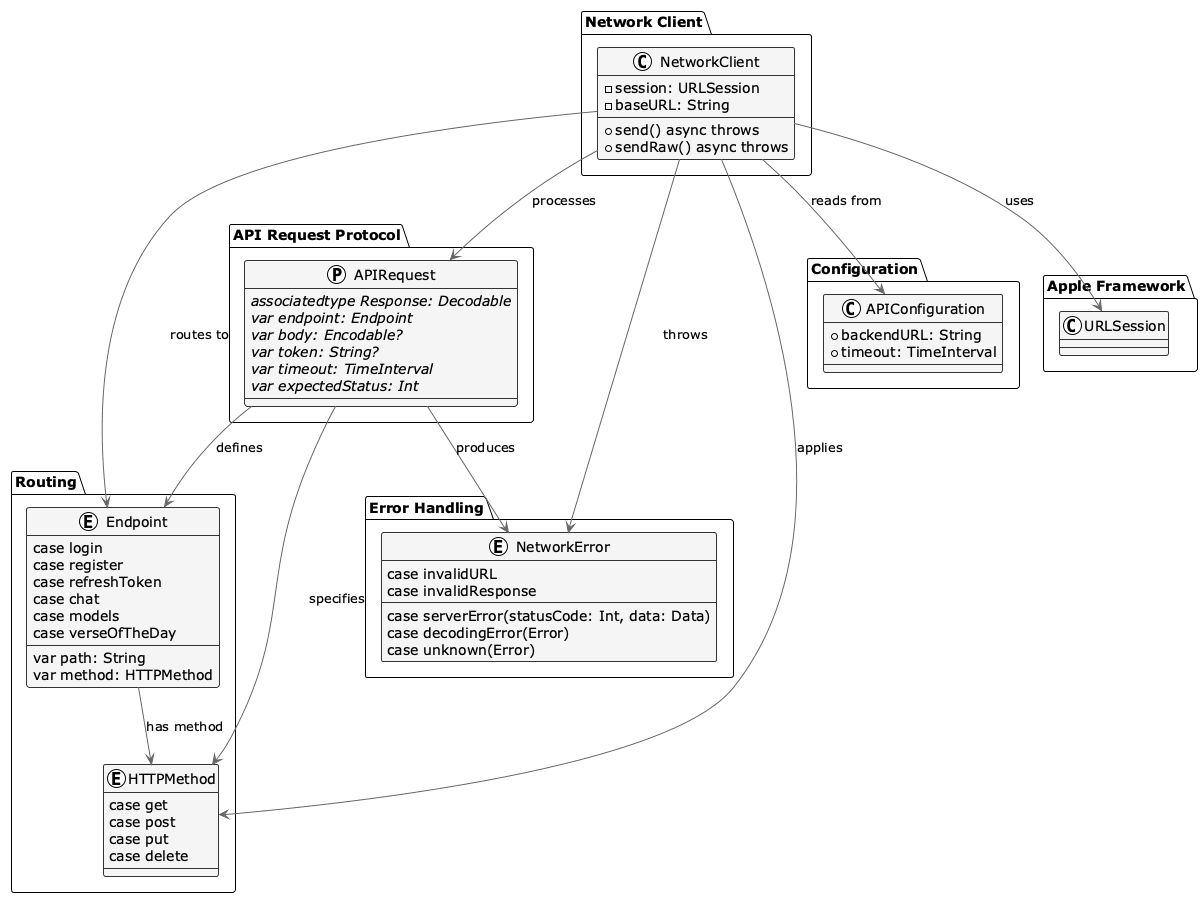
\includegraphics[width=0.85\linewidth]{my_folder/images/image40}
	\caption{UML-диаграмма классов сетевого слоя}
	\label{fig:40}
\end{figure}

\clearpage
